file:///home/ql/5/AA/report/1/5-research.tex {"mtime":1601673170294,"ctime":1600808005786,"size":1425,"etag":"35ojqs78e1eu","orphaned":false}
\chapter{Экспериментальный раздел}
\label{cha:research}

\section{Примеры работы}
% примеры скриншотами интерфейса

На рисунке приведен пример работы программы.

\begin{figure}[h]
    \centering
    \includegraphics[width=0.6\textwidth]{1/inc/example.png}
    \caption{Примеры работы алгоритмов нахождения растоянии Левенптейна и ДамерауЛевенштейна}
\end{figure}



\section{Результаты тестирования}

Использование фреймворка модульного тестирования в Python: unittest

\begin{figure}[h]
    \centering
    \includegraphics[width=0.8\textwidth]{1/inc/test_result.png}
\end{figure}



\pagebreak
\section{Постановка эксперимента по замеру времени и памяти}

\begin{figure}[ht]
    \centering
    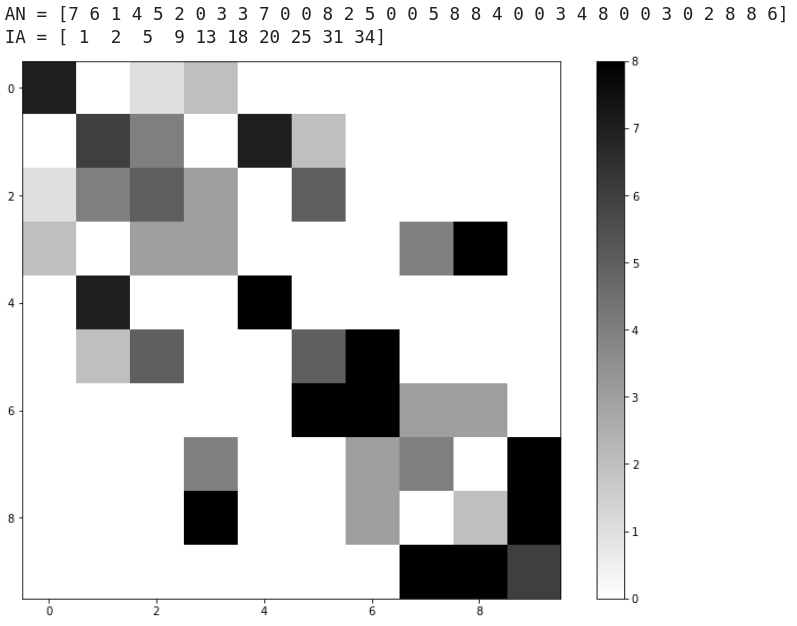
\includegraphics[width=1\textwidth]{1/inc/p1.png}
    \caption{Сравнение времени работы алгоритмов Левенштейна}
\end{figure}

\pagebreak
\begin{figure}[ht]
    \centering
    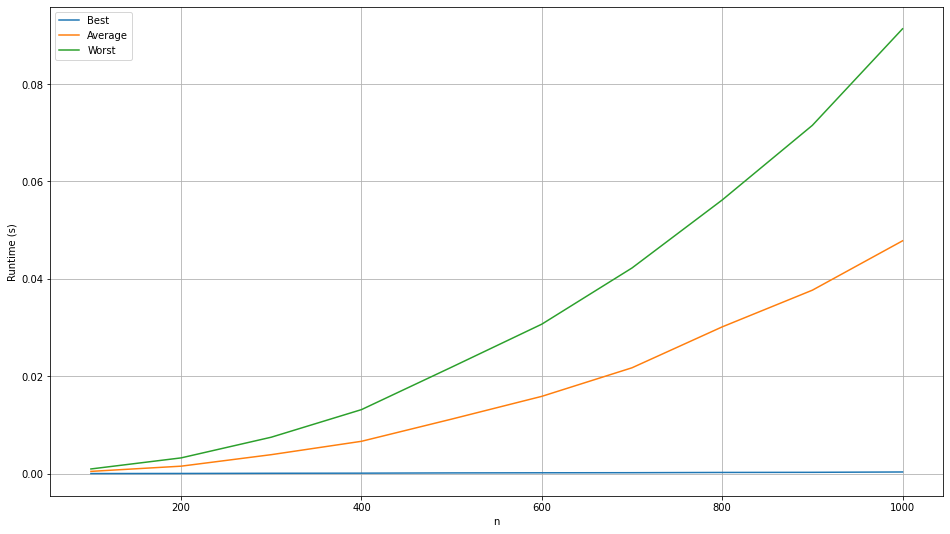
\includegraphics[width=1\textwidth]{1/inc/p2.png}
\end{figure}


\section{Сравнительный анализ на материале экспериментальных данных}
% эксперименты+выводы
